\documentclass[11pt,a4paper]{article}
\usepackage[utf8]{inputenc}
\usepackage[T1]{fontenc}
\usepackage{amsmath, amssymb, amsfonts}
\usepackage{graphicx}
\usepackage{geometry}
\usepackage{booktabs}
\usepackage{xcolor}
\usepackage{hyperref}

\geometry{margin=2.5cm}

\title{\textbf{Technical Report: Neural SDF Architecture for Tactile Reconstruction}}
\author{Tactile-SDF Pipeline}
\date{\today}

\begin{document}

\maketitle

\section{Introduction}
This document details the architecture and loss functions implemented for the 3D reconstruction of objects from sparse tactile contacts. The model maps a set of contact points (position, normal, tangent) to a continuous Signed Distance Function (SDF) representation.

\section{Architecture Overview}
The model follows a \textbf{Conditional Implicit Representation} framework, consisting of a permutation-invariant encoder and a periodic implicit decoder.

\begin{figure}[h]
    \centering
    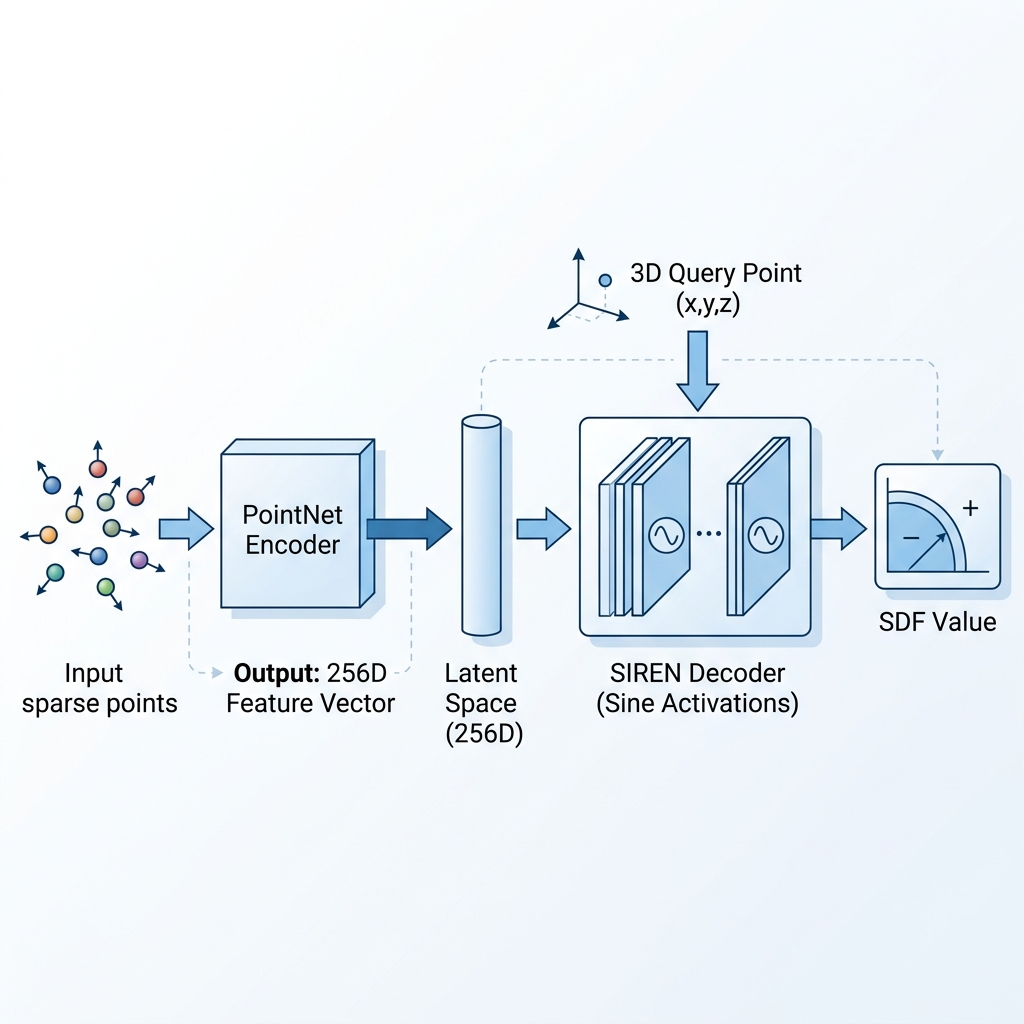
\includegraphics[width=0.9\textwidth]{figures/architecture.png}
    \caption{PointNet + SIREN architecture for tactile SDF reconstruction.}
    \label{fig:arch}
\end{figure}

\subsection{Encoder: PointNet}
To handle an arbitrary number of contact points while being invariant to their order, we use a \textbf{PointNet}-style architecture.
\begin{itemize}
    \item \textbf{Input}: $N$ points $\in \mathbb{R}^9$ (Position $xyz$, Normal $n_{xyz}$, Tangent $t_{xyz}$).
    \item \textbf{Geometric Alignment}: To ensure canonical representation, we compute the object's principal axis via Principal Component Analysis (PCA). The contact positions are normalized relative to this axis, allowing the model to focus on local geometric features rather than global orientation.
    \item \textbf{Layers}: 
        \begin{enumerate}
            \item MLP: $(9 \to 64 \to 128 \to 256)$ with LayerNorm and ReLU.
            \item Global Max Pooling: Reduces the sequence to a single global latent vector.
            \item Latent Projection: MLP $(256 \to 256)$ to produce the final latent code $\mathbf{z}$.
        \end{enumerate}
    \item \textbf{Output}: Latent vector $\mathbf{z} \in \mathbb{R}^{256}$.
\end{itemize}

\subsection{Decoder: SIREN (Sinusoidal Representation Network)}
The decoder is a continuous function $f_\theta(\mathbf{p}, \mathbf{z}) \to s$, where $\mathbf{p}$ is a query coordinate and $s$ is the predicted SDF value. We use \textbf{SIREN} layers because their periodic activation functions are superior for representing complex geometries and their derivatives.

The activation function for each layer is:
\begin{equation}
    \phi(x) = \sin(\omega_0 \cdot x)
\end{equation}
where $\omega_0 = 30$ is a frequency scaling factor.

\begin{itemize}
    \item \textbf{Input}: Concatenation of Query Point $\mathbf{p} \in \mathbb{R}^3$ and Latent Code $\mathbf{z} \in \mathbb{R}^{256}$.
    \item \textbf{Hidden Layers}: 4 layers of width 256 with Sine activations.
    \item \textbf{Output}: Scalar value $s \in \mathbb{R}$ (SDF).
\end{itemize}

\section{Loss Functions}
The model is trained using a weighted sum of three loss components to ensure geometric accuracy and physical consistency.

\subsection{SDF Supervision Loss ($L_{sdf}$)}
Standard L1 loss between predicted and ground-truth SDF values sampled from the mesh.
\begin{equation}
    L_{sdf} = \mathbb{E}_{\mathbf{p}} [ | f_\theta(\mathbf{p}, \mathbf{z}) - SDF_{gt}(\mathbf{p}) | ]
\end{equation}

\subsection{Contact Constraint ($L_{contact}$)}
Forces the surface to pass exactly through the known tactile contact positions $\mathbf{c}_i$.
\begin{equation}
    L_{contact} = \frac{1}{N} \sum_{i=1}^N | f_\theta(\mathbf{c}_i, \mathbf{z}) |
\end{equation}

\subsection{Eikonal Regularization ($L_{eikonal}$)}
Enforces the fundamental property of Signed Distance Functions, where the gradient magnitude must be unity everywhere.
\begin{equation}
    L_{eikonal} = \mathbb{E}_{\mathbf{p}} [ (||\nabla_{\mathbf{p}} f_\theta(\mathbf{p}, \mathbf{z})||_2 - 1)^2 ]
\end{equation}
This loss is computed using automatic differentiation through the SIREN decoder.

\section{Overfitting Mitigation}
To improve generalization and prevent the model from memorizing specific contact coordinates, we implement two key strategies:

\subsection{Dataset Expansion}
The dataset is expanded from 50 to 100 objects (20 per category), with multiple grasp strategies per object. This increases the total sample count and forces the encoder to learn more diverse structural priors.

\subsection{Tactile Data Augmentation}
During training, we apply online data augmentation to the contact points. Each contact position $\mathbf{c}_i$ is perturbed by additive Gaussian noise:
\begin{equation}
    \mathbf{c}'_i = \mathbf{c}_i + \epsilon, \quad \epsilon \sim \mathcal{N}(0, \sigma^2)
\end{equation}
where $\sigma = 0.005$ in normalized coordinates. This ensures the model learns to be robust to small sensor errors and improves reconstruction stability.

\section{Summary Table}
\begin{table}[h]
    \centering
    \begin{tabular}{lll}
        \toprule
        \textbf{Component} & \textbf{Type} & \textbf{Hyperparameters} \\
        \midrule
        Encoder & PointNet & Latent Dim: 256 \\
        Decoder & SIREN & Layers: 4, Width: 256, $\omega_0$: 30 \\
        Optimizer & Adam & LR: $1 \times 10^{-4}$, Cosine Schedule \\
        Loss Weight & $\lambda_{contact}$ & 0.1 \\
        Loss Weight & $\lambda_{eikonal}$ & 0.01 \\
        \bottomrule
    \end{tabular}
    \caption{Architecture and Training Hyperparameters}
\end{table}

\end{document}
